% $Header: /cvsroot/latex-beamer/latex-beamer/solutions/conference-talks/conference-ornate-20min.en.tex,v 1.7 2007/01/28 20:48:23 tantau Exp $

\documentclass[aspectratio=169]{beamer}

\mode<presentation>
{
  %% \usetheme{Rochester}
  %% \usetheme{AnnArbor}
  %% \usetheme{Madrid}
  %% \usetheme{Malmoe}
  %% \usetheme{PaloAlto}
  \usetheme{Marburg}            % contents, title
  %% \usetheme{Montpellier}        % o
  %% \usetheme{Warsaw}
  %% \usetheme{Berlin}
  %% \usetheme{Singapore}
  %% \usetheme{Bergen}
  %% \usetheme{Pittsburgh}
  %% \usetheme{Dresden}
  %% \usetheme{Darmstadt}
  %% \usetheme{Frankfurt}
  %% \usetheme{Antibes}            %similar to montpellier
  %% \usetheme{Hannover}           % similar to marburg
  %% \usetheme{Copenhagen}
  %% \usetheme{JuanLesPins}
  %% \usetheme{Szeged}
  %% \usetheme{Berkeley}
  %% \usetheme{CambridgeUS}
  %% \usetheme{Ilmenau}
  %% \usetheme{Boadilla}
  %% \usetheme{Goettingen}         %similar to hannover
  %% \usetheme{Luebeck}
  % or ...
  \setbeamercovered{transparent}
  % or whatever (possibly just delete it)
}

%% \usepackage[orientation=landscape,size=custom,width=16,height=9.75,scale=0.5,debug]{beamerposter}
\usepackage{fontspec}
%% \newfontfamily\zhfont{KaiTi}
\usepackage{zhspacing}
\zhspacing
\usepackage{amsmath}
\usepackage{listings}
\usepackage{subfigure}
\usepackage{asymptote}
%% \newcommand{\ppbox}[1]{\vbox to .2\textwidth{\vfil\hbox to .2\textwidth{#1}\vfil}}
\newcommand{\ppbox}[3]{\vbox to #1{\vfil\hbox to #2{#3}\vfil}}
\newcommand{\vvbox}[2]{\vbox to #1{\vfil{#2}\vfil}}
%% \usepackage[english]{babel}
% or whatever
%% \usepackage[latin1]{inputenc}
% or whatever
%% \usepackage{times}
%% \usepackage[T1]{fontenc}
% Or whatever. Note that the encoding and the font should match. If T1
% does not look nice, try deleting the line with the fontenc.

\title[并行处理器稠密线性代数数学库]{面向并行处理器的稠密线性代数数学库\\关键技术研究}

%% \subtitle
%% {Include Only If Paper Has a Subtitle}

\author[苏醒]{苏醒\inst{1}}
% - Give the names in the same order as the appear in the paper.
% - Use the \inst{?} command only if the authors have different
%   affiliation.

\institute[计算机学院软件所] % (optional, but mostly needed)
{
  \inst{1}
  计算机学院软件所
}
% - Use the \inst command only if there are several affiliations.
% - Keep it simple, no one is interested in your street address.

%% \date[CFP 2003] % (optional, should be abbreviation of conference name)
%% {Conference on Fabulous Presentations, 2003}
%% \renewcommand{\today}{\number\year{}年{}\number\month{}月{}\number\day{}日}
\date{\number\year{}年{}\number\month{}月{}\number\day{}日}
% - Either use conference name or its abbreviation.
% - Not really informative to the audience, more for people (including
%   yourself) who are reading the slides online

%% \subject{Theoretical Computer Science}
% This is only inserted into the PDF information catalog. Can be left
% out. 



% If you have a file called "university-logo-filename.xxx", where xxx
% is a graphic format that can be processed by latex or pdflatex,
% resp., then you can add a logo as follows:

\pgfdeclareimage[height=1cm]{nudt-logo}{nudtlogo1}
\logo{\pgfuseimage{nudt-logo}}


% Delete this, if you do not want the table of contents to pop up at
% the beginning of each subsection:
\AtBeginSubsection[]
{
  \begin{frame}<beamer>{内容}
    \tableofcontents[currentsection,currentsubsection]
  \end{frame}
}


% If you wish to uncover everything in a step-wise fashion, uncomment
% the following command: 

%\beamerdefaultoverlayspecification{<+->}


\begin{document}

%% \def\asylatexdir{asylatex}
%% \def\asydir{asy}
\begin{asydef}
  import matrix;
\end{asydef}

\begin{frame}
  \titlepage
\end{frame}

\begin{frame}{内容}
  \tableofcontents
  % You might wish to add the option [pausesections]
\end{frame}


% Structuring a talk is a difficult task and the following structure
% may not be suitable. Here are some rules that apply for this
% solution: 

% - Exactly two or three sections (other than the summary).
% - At *most* three subsections per section.
% - Talk about 30s to 2min per frame. So there should be between about
%   15 and 30 frames, all told.

% - A conference audience is likely to know very little of what you
%   are going to talk about. So *simplify*!
% - In a 20min talk, getting the main ideas across is hard
%   enough. Leave out details, even if it means being less precise than
%   you think necessary.
% - If you omit details that are vital to the proof/implementation,
%   just say so once. Everybody will be happy with that.

\section{研究背景}

\subsection[重要性]{线性代数数学库的重要性}

\begin{frame}
  \frametitle{数值线性代数问题}
  \begin{itemize}
  \item 科学与工程计算中最重要的一类数值计算问题
    \begin{itemize}
    \item 线性方程组求解
    \item 线性最小二乘问题
    \item 矩阵特征值问题
    \end{itemize}
  \item 根据涉及矩阵的性质可以分为两类
    \begin{itemize}
    \item 稠密类问题(矩阵大多数元素非0)
    \item 稀疏类问题(矩阵大多数元素为0)
    \end{itemize}
  \end{itemize}
\end{frame}

\begin{frame}
  \frametitle{数值线性代数的应用}
  \begin{itemize}
  \item 广泛应用于科学与工程计算的各个领域
    \begin{itemize}
    \item 数值天气预报
    \item 石油勘探
    \item 地震数据处理
    \item 核模拟
    \item 生命科学
    \end{itemize}
  \item 高性能计算领域的主要benchmark
    \begin{itemize}
    \item LINPACK
    \item HPCG
    \end{itemize}
  \end{itemize}
\end{frame}

\begin{frame}
  \frametitle{线性代数数学库}
  \begin{itemize}
  \item 鉴于数值线性代数的重要性,其常用函数通常被封装成高性能程序库
    \begin{itemize}
    \item BLAS
    \item LINPACK/EISPACK/LAPACK
    \end{itemize}
  \item 本课题主要关心稠密线性代数数学库
  \end{itemize}
\end{frame}

\subsection[体系结构]{处理器体系结构发展现状}

\begin{frame}
  \frametitle{多层次的并行计算能力}
  \framesubtitle{指令级并行}
  \begin{itemize}
  \item 流水线
  \item 多发射
  \item 动态调度
  \item 乱序执行
  \end{itemize}
\end{frame}

\begin{frame}
  \frametitle{多层次的并行计算能力}
  \framesubtitle{数据级并行}
  \begin{itemize}
  \item SIMD指令
    \begin{itemize}
    \item X86
      \begin{itemize}
      \item MMX/SSE/SSE2/SSE3/SSE4/AVX/AVX2/AVX512
      \end{itemize}
    \item ARM
      \begin{itemize}
      \item NEON
      \end{itemize}
    \end{itemize}
  \end{itemize}
  \begin{figure}
    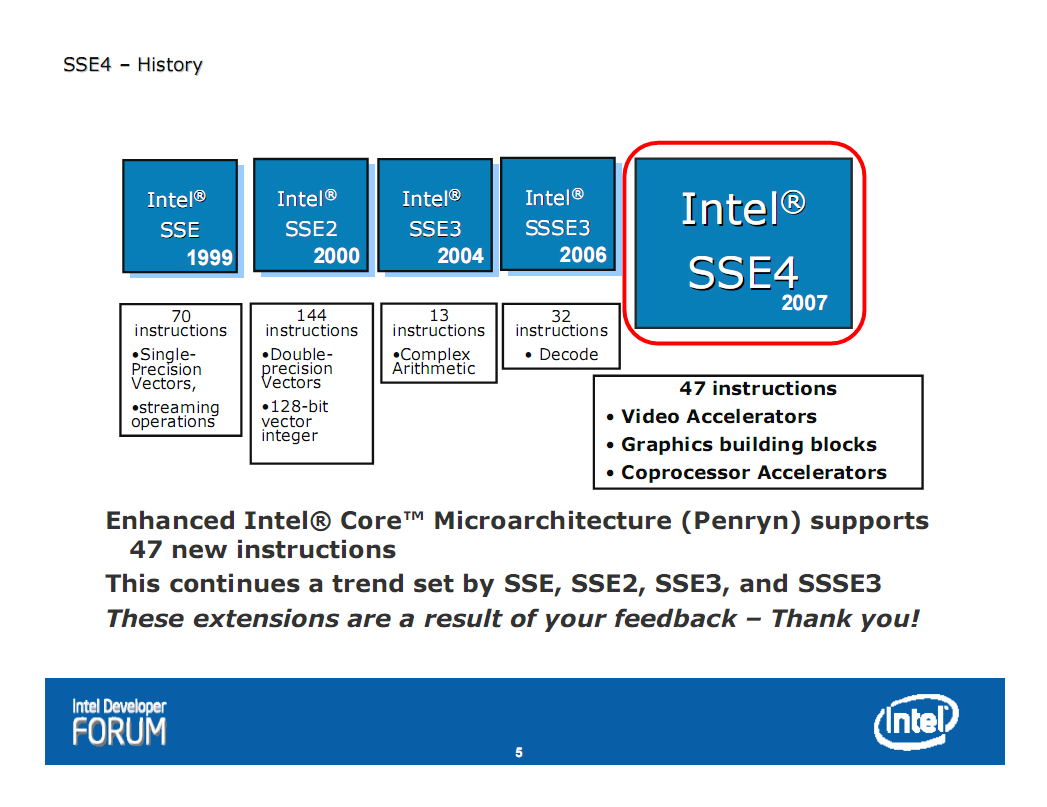
\includegraphics[width=.4\textwidth]{intel-simd}\hspace{1cm}
    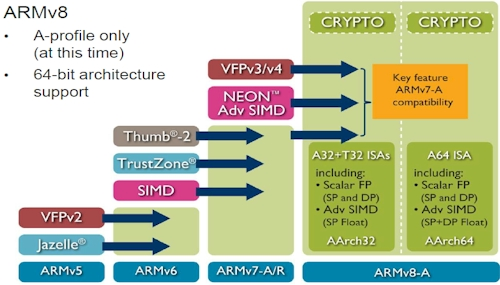
\includegraphics[width=.4\textwidth]{arm-simd}
  \end{figure}
\end{frame}

\begin{frame}
  \frametitle{多层次的并行计算能力}
  \framesubtitle{线程级并行}
  \begin{itemize}
  \item 多核处理器的主流地位
    \begin{itemize}
    \item 单核计算能力瓶颈
    \end{itemize}
  \item 众核(协)处理器的发展趋势
    \begin{itemize}
    \item 日益增长的计算能力需求
    \end{itemize}
  \end{itemize}
  \begin{figure}
    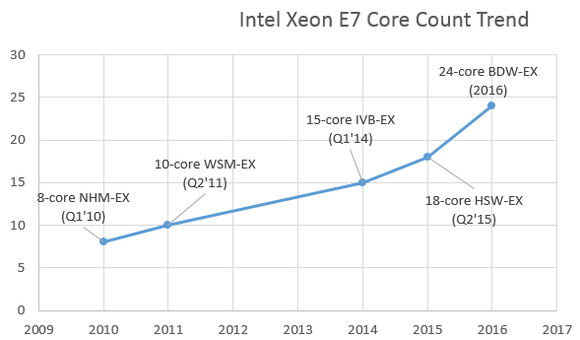
\includegraphics[width=.4\textwidth]{e7}\hspace{1cm}
    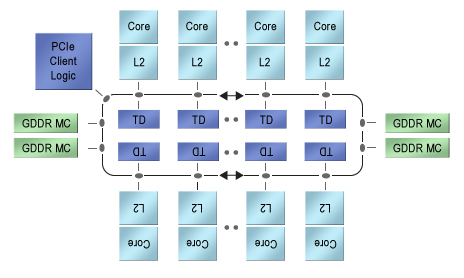
\includegraphics[width=.4\textwidth]{knc1}
  \end{figure}
  %% include figure demonstrating the increasing trend of on-chip cores
\end{frame}

\begin{frame}
  \frametitle{多样化的存储层次结构}
  \begin{itemize}
  \item “存储墙”:存储器速度增长落后于计算能力增长 % figure
  \item 存储层次结构趋于复杂
    \begin{itemize}
    \item inclusive/exclusive
    \item 互联网络实现的一致性
    \item 非一致性cache访问(NUCA)
    \end{itemize}
  \end{itemize}
  \begin{figure}
    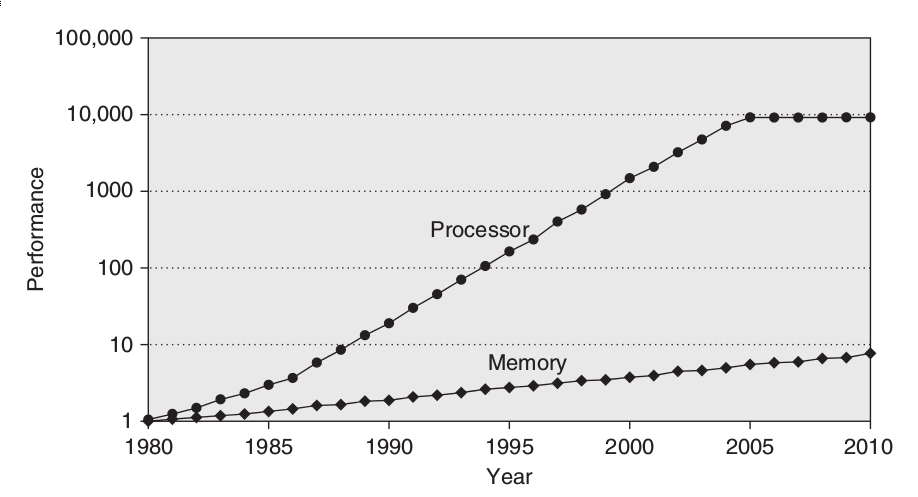
\includegraphics[width=.4\textwidth]{cpu-mem-gap}\hspace{1cm}
    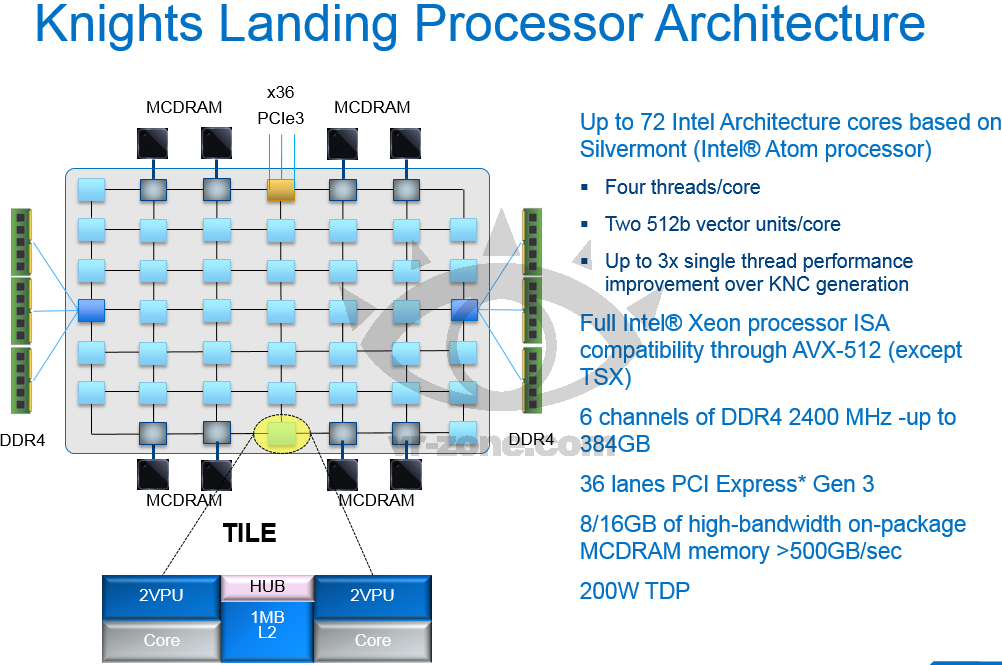
\includegraphics[width=.4\textwidth]{knl}
  \end{figure}
\end{frame}

\subsection[研发现状]{稠密线性代数数学库的研究发展现状}

\begin{frame}
  \frametitle{发展历程}
  \begin{itemize}
  \item (准)标准接口
    \begin{itemize}             %figure instead?
    \item BLAS(1970s-1980s)
    \item EISPACK(1970s-1980s)
    \item LINPACK(1970s-1980s)
    \item LAPACK(1990s)
    \end{itemize}
  \end{itemize}
\end{frame}

\begin{frame}
  \frametitle{实现技术}
  \begin{itemize}
  \item 基于矩阵乘法(GEMM)的BLAS实现
  \item 基于BLAS的LAPACK实现
  \item 高性能GEMM的实现方法
    \begin{itemize}
    \item 通过矩阵分块有效利用cache
    \item 通过子任务调度开发线程级并行
    \item 使用SIMD指令取得峰值浮点性能
    \end{itemize}
  \end{itemize}
  \includegraphics[width=.6\textwidth]{lib-hierachy}
\end{frame}

\begin{frame}
  \frametitle{问题与挑战}
  \framesubtitle{GEMM最优性能严重平台相关}
  \begin{columns}
    \begin{column}{.5\textwidth}
      \begin{itemize}
      \item kernel函数实现
        \begin{itemize}
        \item 寄存器分配
        \item 指令调度
        \end{itemize}
      \item 分块策略
        \begin{itemize}
        \item 维度选择
        \item 分块大小
        \end{itemize}
      \item 调度策略
        \begin{itemize}
        \item 并行粒度
        \item 执行顺序
        \end{itemize}
      \end{itemize}
    \end{column}
    \begin{column}{.5\textwidth}
      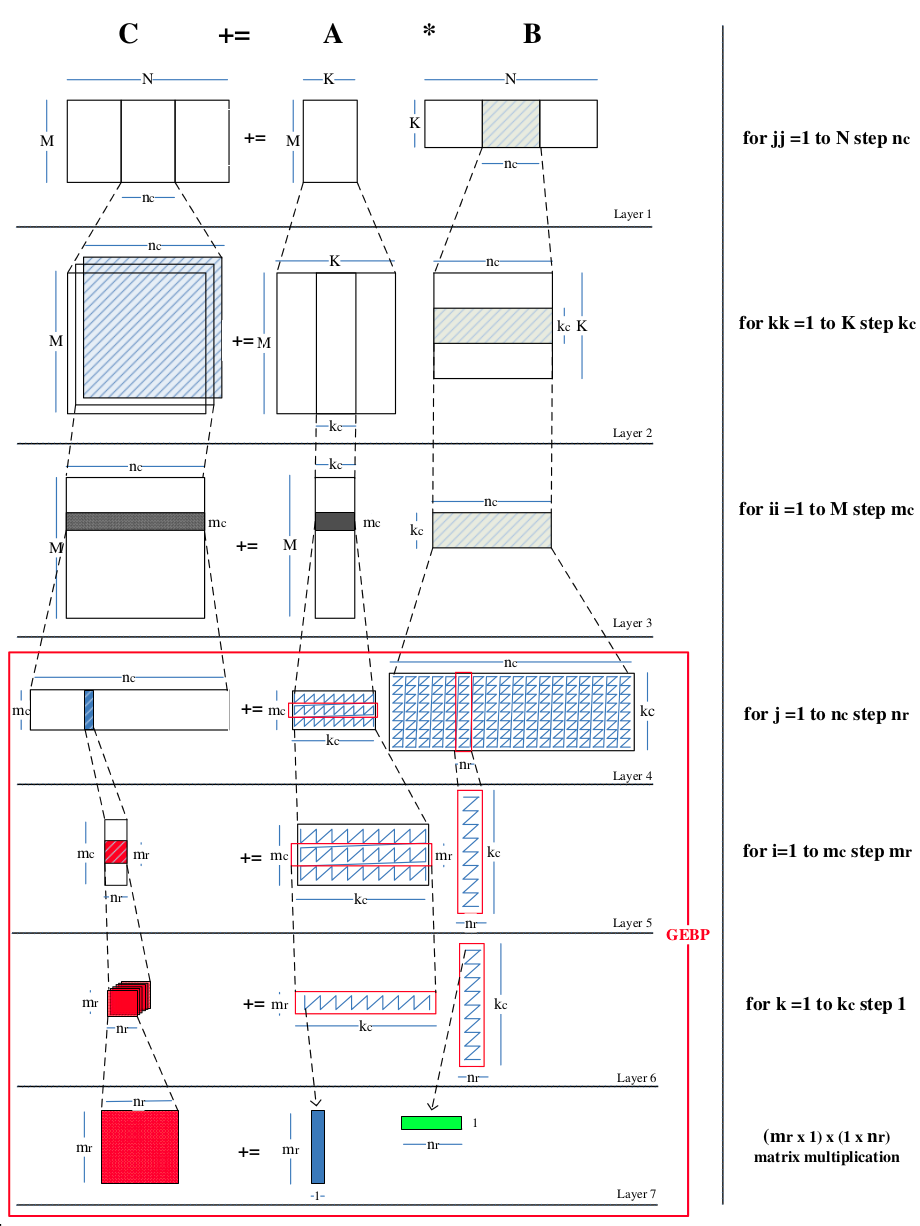
\includegraphics[width=.8\textwidth]{gemm}
    \end{column}
  \end{columns}
\end{frame}

\begin{frame}
  \frametitle{问题与挑战}
  \framesubtitle{众核平台上的并行可扩展性}
  \begin{columns}
    \begin{column}{.4\textwidth}
      \begin{itemize}
      \item 更高的线程并行度
        \begin{itemize}
        \item 多核/众核
        \item 超线程
        \end{itemize}
      \item 更复杂的存储层次结构
        \begin{itemize}
        \item 一致性对性能的影响
        \item NUCA对性能的影响
        \end{itemize}
      \end{itemize}
    \end{column}
    \begin{column}{.6\textwidth}
      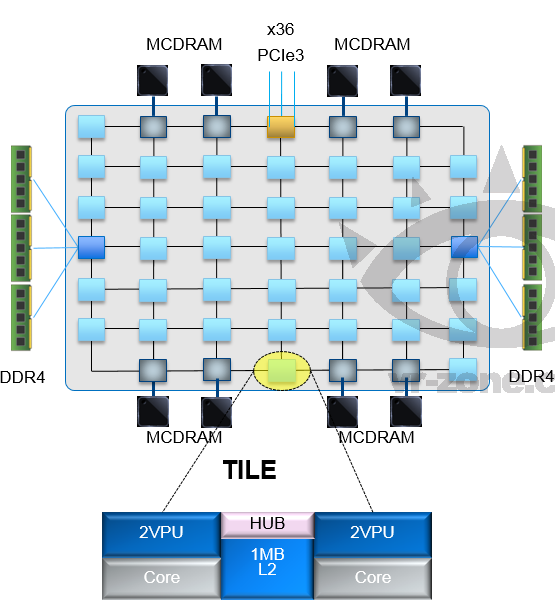
\includegraphics[width=.7\textwidth]{knl1}
    \end{column}
  \end{columns}
\end{frame}

\begin{frame}
  \frametitle{问题与挑战}
  \framesubtitle{全局优化缺失}
  \begin{itemize}
  \item 高性能库函数的逐级调用构成完整应用程序
    \begin{itemize}
    \item 模块化程度高
    \item 性能优化控制在单层级
    \end{itemize}
  \item 无跨层级的全局优化
  \end{itemize}
\end{frame}

\begin{frame}
  \frametitle{问题与挑战}
  \framesubtitle{现有(准)标准接口限制}
  \begin{itemize}
  \item 现有BLAS/LAPACK接口设计不够完善
    \begin{itemize}
    \item 跨类型操作
    \item 非连续存储
    \end{itemize}
  \item 额外的数据拷贝与转存造成性能损失
  \end{itemize}
\end{frame}

\section{研究内容}

\begin{frame}
  \frametitle{研究内容}
  \begin{itemize}
  \item 针对稠密线性代数运算的编译优化技术研究
  \item 面向众核处理器的并行优化技术研究
  \item 适用于一般稠密线性代数问题的全局优化技术研究
  \item 面向稠密线性代数的领域语言研究
  \end{itemize}
\end{frame}

\subsection[编译优化技术研究]{针对稠密线性代数运算的编译优化技术研究}

\begin{frame}
  \frametitle{针对稠密线性代数运算的编译优化技术研究}
  \begin{itemize}
  \item 问题描述
    \begin{itemize}
    \item 稠密线性代数程序存在若干核心kernel函数
      \begin{itemize}
      \item GEMM/GEMV
      \item TRSM/TRSV
      \end{itemize}
    \item kernel函数是程序整体性能的决定性因素之一
    \item kernel函数的最优实现严重平台相关
    \end{itemize}
  \item 研究现状
    \begin{itemize}
    \item 专家编写汇编代码
      \begin{itemize}
      \item GotoBLAS/OpenBLAS
      \end{itemize}
    \item 代码自动生成与调优
      \begin{itemize}
      \item ATLAS
      \end{itemize}
    \item 基于pattern的编译优化
      \begin{itemize}
      \item AUGEM(OpenBLAS)
      \end{itemize}
    \item 经典编译技术
      \begin{itemize}
      \item BLIS
      \end{itemize}
    \end{itemize}
  \end{itemize}
\end{frame}

\begin{frame}
  \frametitle{针对稠密线性代数运算的编译优化技术研究}
  \begin{itemize}
  \item 研究思路
    \begin{itemize}
    \item 总结专家知识,定位影响性能的关键要素
      \begin{itemize}
      \item 体系结构特性:核心指令种类、延迟、处理器部件占用情况等
      \item 微体系结构特性:指令调度器、功能部件种类及数目等
      \end{itemize}
    \item 基于开源编译器框架,实现针对kernel函数的最优代码生成
    \end{itemize}
  \item 预期创新点
    \begin{itemize}
    \item 针对稠密线性代数问题的编译优化技术
    \end{itemize}
  \end{itemize}
\end{frame}

\subsection[并行可扩展性研究]{面向众核处理器的并行优化技术研究}

\begin{frame}
  \frametitle{面向众核处理器的并行优化技术研究}
  \begin{itemize}
  \item 问题描述
    \begin{itemize}
    \item 线程级并行度进一步提高,现有分块与调度策略需要调整
      \begin{itemize}
      \item 超线程
      \item 一维并行划分可扩展性差
      \end{itemize}
    \item 众核处理器不符合简单的inclusive cache存储层次结构模型
      \begin{itemize}
      \item 小容量exclusive LLC(FT series)
      \item 网络互联cache(KNC/KNL)
      \end{itemize}
    \end{itemize}
  \item 研究现状
    \begin{itemize}
    \item 自动调优选择分块大小
      \begin{itemize}
      \item ATLAS
      \end{itemize}
    \item 分析方法选择分块大小
      \begin{itemize}
      \item BLIS
      \end{itemize}
    \item 编译指导代码变换
      \begin{itemize}
      \item POET
      \end{itemize}
    \item 二维并行代替一维并行
      \begin{itemize}
      \item BLIS
      \end{itemize}
    \end{itemize}
  \end{itemize}
\end{frame}

\begin{frame}
  \frametitle{面向众核处理器的并行优化技术研究}
  \begin{itemize}
  \item 研究思路
    \begin{itemize}
    \item 最优划分调度策略主要由存储体系结构特性决定
      \begin{itemize}
      \item 拓扑
      \item 一致性协议
      \end{itemize}
    \item 分层考虑存储层次结构中的计算与数据传输过程,
      \begin{itemize}
      \item 下层存储器根据上层存储器特性进行任务划分
      \item 上层存储器对下层存储器提交的任务进行调度
      \end{itemize}
    \end{itemize}
  \item 预期创新点
    \begin{itemize}
    \item 用于商用众核处理器KNC/KNL及国产飞腾众核处理器并行优化技术
    \item 适用于复杂存储层次结构的的性能分析模型
    %% \item 性能分析模型下的整体优化策略自动生成
    \end{itemize}
  \end{itemize}
\end{frame}

\subsection[全局优化技术研究]{一般稠密线性代数问题的全局优化技术研究}

\begin{frame}
  \frametitle{一般稠密线性代数问题的全局优化技术研究}
  \begin{itemize}
  \item 问题描述
    \begin{itemize}
    \item 通过组合库函数调用的方式编写程序缺乏全局优化 %example
    \item 函数库的接口限制造成的数据拷贝、转存附加开销
    \end{itemize}
  \item 研究现状
    \begin{itemize}
    \item 全局优化方面暂时未见相关研究
    \item 在GEMM实现内部的pack/unpack过程中加入对跨类型运算与非连续存储的支持
      \begin{itemize}
      \item BLIS(初探阶段,尚未实现)
      \end{itemize}
    \end{itemize}
  \end{itemize}
\end{frame}

\begin{frame}
  \frametitle{一般稠密线性代数问题的全局优化技术研究}
  \begin{itemize}
  \item 研究思路
    \begin{itemize}
    \item 常见的稠密线性代数问题的求解可以通过少量基本矩阵操作组合得到
      \begin{itemize}
      \item 逐点操作
      \item 规约操作
      \item 矩阵乘法
      \item 高斯消元
      \end{itemize}
    \item 算法层面上,稠密线性代数运算多数可以采用分块递归的形式描述
      \begin{itemize}
      \item 适合在存储层次结构上作分块映射
      \end{itemize}
    \item 基于上一研究点提出的性能分析模型提出全局优化方法
    \item 全局优化过程中选择合适的存储层次执行数据拷贝与转存,最小化性能损失
    \end{itemize}
  \item 预期创新点
    \begin{itemize}
    \item 适用于一般的稠密线性代数问题的全局优化技术
    \end{itemize}
  \end{itemize}
\end{frame}

\subsection[领域语言研究]{面向稠密线性代数的领域语言研究}

\begin{frame}
  \frametitle{面向稠密线性代数的领域语言研究}
  \begin{itemize}
  \item 问题描述
    \begin{itemize}
    \item 现有的高性能数学库一般使用FORTRAN与C语言编写
      \begin{itemize}
      \item 编写难度大,维护成本高
      \item 性能可移植性差
      \end{itemize}
    \end{itemize}
  \item 研究现状
    \begin{itemize}
    \item 领域语言与编译技术
      \begin{itemize}
      \item LGen(只应用于嵌入式应用的小规模矩阵计算)
      \end{itemize}
    \item 面向科学计算的脚本语言与库
      \begin{itemize}
      \item Matlab/Octave/NumPy
      \item 低层仍依赖BLAS/LAPCK
      \end{itemize}
    \end{itemize}
  \end{itemize}
\end{frame}

\begin{frame}
  \frametitle{面向稠密线性代数的领域语言研究}
  \begin{itemize}
  \item 研究思路
    \begin{itemize}
    \item 基于前述的研究内容,设计面向大规模稠密线性代数的领域语言
      \begin{itemize}
      \item 抽象层次高,表达简洁
      \item 符合现代处理器体系结构特点,易于映射
      \item 支持C语言调用
      \end{itemize}
    \end{itemize}
  \item 预期创新点
    \begin{itemize}
    \item 面向稠密线性代数的领域语言的设计与实现
    \end{itemize}
  \end{itemize}
\end{frame}

\section{研究基础}

\begin{frame}
  \frametitle{研究基础}
  \begin{itemize}
  \item 课题组在优化高性能数学库方面有持续性投入
  \item 熟悉高性能矩阵乘法实现的关键优化技术,了解现有开源BLAS库的开发现状
  \item 具备编译知识基础,有能力基于开源编译器LLVM的进行开发
  \item 接受新南威尔士大学薛京灵教授指导,薛教授是编译领域资深专家
  \item 课题组可以提供优秀的实验环境与设备
  \end{itemize}
\end{frame}

\section{预期成果}

\begin{frame}
  \frametitle{预期成果}
  \begin{itemize}
  \item 针对稠密线性代数问题的编译优化技术
  \item 面向众核平台复杂存储层次结构的并行优化技术
  \item 适用于一般稠密线性代数问题的全局优化技术
  \item 稠密线性代数领域语言的设计与实现
  \end{itemize}
\end{frame}

\section{时间安排}

\begin{frame}
  \frametitle{时间安排}
  \begin{table}
    \footnotesize{
    \begin{tabular}{l|p{.4\textwidth}|l}
      \hline
      \textbf{时间}   & \textbf{内容}                            & \textbf{预期成果} \\
      \hline
      2016.01-2016.04 & 稠密线性代数问题的编译优化技术           & 基于LLVM的实现 \\
      2016.05-2016.07 & 适用于复杂存储层次的分块调度优化策略     & 会议论文一篇 \\
      2016.08-2016.12 & 为一般稠密线性代数问题提供自动化实现技术 & 会议论文一篇 \\
      2017.01-2017.05 & 设计实现面向稠密线性代数的领域语言       & 期刊论文一篇 \\
      2017.06-2017.10 & 完善已有实验,完善项目代码,撰写博士论文 & 完整工程项目 \\
      2017.11-1017.11 & 修改博士论文,答辩                       & 博士论文 \\
      \hline
    \end{tabular}}
  \end{table}
\end{frame}

\section*{总结}

\begin{frame}
  \frametitle{总结}
  \begin{itemize}
    \item 优化成本是数稠密性代数数学库研发中的主要挑战
    \item 处理器体系结构的快速发展要求更好自动优化方法
    \item 本课题的目标是为高性能稠密线性代数数学库提出一套完整解决方案
      \begin{itemize}
      \item 针对稠密线性代数问题的编译优化技术
      \item 面向众核平台复杂存储层次结构的并行优化技术
      \item 适用于一般稠密线性代数问题的全局优化技术
      \item 稠密线性代数领域语言的设计与实现
      \end{itemize}
  \end{itemize}
\end{frame}

\begin{frame}
  %% \begin{itemize}
  %%   \item 前两个点都是做GEMM,是否作为一个点才比较丰满?
  %%   \item 全局优化是否值得做,还没有系统调研
  %%   \item 开题报告slides存在那些问题
  %%   \item 开题报告的撰写要注意那些问题
  %% \end{itemize}
  \centerline{\Huge{请各位老师批评指正!}}
\end{frame}

\AtBeginSubsection[]{}          % disable TOC

\appendix
\section<presentation>*{\appendixname}
\subsection<presentation>*{Global Optimization}

\begin{frame}
  \frametitle{Global Optimization}
  \framesubtitle{An Example}
  \begin{itemize}
  \item We use the \alert{LU factorization with partial pivoting} algorithm
    as a running example to demonstrate some details of global optimization
  \end{itemize}
  \begin{block}{LU Factorization with partial pivoting}
    Given a square matrix $A \in \mathbf{R^{n \times n}}$, there exists a
    row permutation matrix $P$, a unit lower triangular matrix $L$ and a upper
    triangular matrix $U$ such that
    $$PA=LU$$
  \end{block}
\end{frame}

\begin{frame}
  \frametitle{LU Factorization with Partial Pivoting}
  \framesubtitle{A Simple Machine Architecture}
  \begin{columns}
    \begin{column}{.6\textwidth}
      \begin{itemize}
      \item For convenience, we assume a simple machine architecture
        \begin{itemize}
        \item 1 CPU core
        \item 1 level cache
        \end{itemize}
      \item The blocked algorithm should be used to better utilize cache memory
      \end{itemize}
    \end{column}
    \begin{column}{.4\textwidth}
      \begin{figure}
        \centering
        \includegraphics[width=.8\textwidth]{machine}
      \end{figure}
    \end{column}
  \end{columns}
\end{frame}

\begin{frame}[fragile]
  \frametitle{LU Factorization with Partial Pivoting}
  \framesubtitle{The Recursive Algorithm}
  \begin{columns}
    \begin{column}{.5\textwidth}
      \setbeamerfont{code}{size=\scriptsize}
      \begin{semiverbatim}
        \usebeamerfont{code}
        \uncover<1->{\alert<1>{void LU(A) \{}}
        \uncover<2->{\alert<2,9>{  [A0 | A1] = A}}
        \uncover<3->{\alert<3,10>{  (U00, L0, P0) = GAUSSIAN(A0)}}
        \uncover<4->{\alert<4,10>{  A1 = P * A1}}
        \uncover<5->{\alert<5,11>{  [L00; L10] = L0}}
        \uncover<5->{\alert<5,11>{  [A01; A11] = A1}}
        \uncover<6->{\alert<6,12>{  U01 = TRSM(L00, A01)}}
        \uncover<7->{\alert<7,12>{  A11 = GEMM(L10, U01, A11)}}
        \uncover<8->{\alert<8,13>{  (L11, U11) = LU(A11)}}
        \uncover<1->{\alert<1>{\}}}
      \end{semiverbatim}
    \end{column}
    \begin{column}{.5\textwidth}
      \centering
      \begin{tabular}{ccc}
        \ppbox{.2\textwidth}{.2\textwidth}{\includegraphics<1->[width=.2\textwidth]{lu0}} &
        \ppbox{.2\textwidth}{.2\textwidth}{\includegraphics<2->[width=.2\textwidth]{lu1}} &
        \ppbox{.2\textwidth}{.2\textwidth}{\includegraphics<3->[width=.2\textwidth]{lu2}} \\
        \ppbox{.2\textwidth}{.2\textwidth}{\includegraphics<5->[width=.2\textwidth]{lu3}} &
        \ppbox{.2\textwidth}{.2\textwidth}{\includegraphics<6->[width=.2\textwidth]{lu4}} &
        \ppbox{.2\textwidth}{.2\textwidth}{\includegraphics<8>[width=.2\textwidth]{lu5}
          \includegraphics<9->[width=.2\textwidth]{lu6}} \\
        \ppbox{.2\textwidth}{.2\textwidth}{\includegraphics<10->[width=.2\textwidth]{lu7}} &
        \ppbox{.2\textwidth}{.2\textwidth}{\includegraphics<11->[width=.2\textwidth]{lu8}} &
        \ppbox{.2\textwidth}{.2\textwidth}{\includegraphics<12->[width=.2\textwidth]{lu9}} \\
        \ppbox{.2\textwidth}{.2\textwidth}{\includegraphics<13->[width=.2\textwidth]{lu10}} & &
      \end{tabular}
    \end{column}
  \end{columns}
\end{frame}

\begin{frame}[fragile]
  \frametitle{LU Factorization with Partial Pivoting}
  \framesubtitle{Dependence and Scheduling}
  \begin{columns}
    \begin{column}{.5\textwidth}
      %% \setbeamerfont{code}{size=\scriptsize}
      %% \begin{semiverbatim}
      %%   \usebeamerfont{code}
      %%   void LU(A) \{
      %%     [A0 | A1] = A
      %%     (U00, L0, P0) = GAUSSIAN(A0)
      %%     A1 = P * A1
      %%     [L00; L10] = L0
      %%     [A01; A11] = A1
      %%     U01 = TRSM(L00, A01)
      %%     A11 = GEMM(L10, U01, A11)
      %%     (L11, U11) = LU(A11)
      %%   \}
      %% \end{semiverbatim}
      \vvbox{.8\textheight}{
      \begin{figure}
        \includegraphics[width=.4\textwidth]{lu11}
      \end{figure}
      }
    \end{column}
    \begin{column}{.5\textwidth}
      \centering
        \includegraphics<1>[width=.3\textwidth]{ludep0}
        \includegraphics<2>[width=.7\textwidth]{ludep1}
        \includegraphics<3>[width=.7\textwidth]{ludep2}
        \includegraphics<4>[width=.7\textwidth]{ludep3}
        \includegraphics<5>[width=.7\textwidth]{ludep4}
        \includegraphics<6>[width=.7\textwidth]{ludep5}
    \end{column}
  \end{columns}
\end{frame}

\begin{frame}
  \frametitle{Global Optimization}
  \framesubtitle{Summary}
  \begin{itemize}
  \item The real world is far more complex
    \begin{itemize}
    \item Applications are far more complex than LU factorization
    \item Modern microprocessor architecture are far more complex than that assumed
    \end{itemize}
  \item Manual optimization is quite labor-intensive
  \item Dense linear algebra is a class of problems with good properties,
    making it possible for developing automatic optimizing techniques
    \begin{itemize}
    \item computationally intensive
    \item regular datasets
    \item good parallelism
    \end{itemize}
  \end{itemize}
\end{frame}


%% \begin{frame}
%%   \frametitle{An Example of Global Optimization}
%%   \begin{itemize}
%%     \item We use the Cholesky factorization of symmetric positive definite matrix
%%       as a running example to demonstrate some details of global optimization
%%   \end{itemize}
%%   \begin{theorem}
%%     (Cholesky Factorization)
%%     If $A \in \boldsymbol{R}^{n \times n}$ is symmetric positive details,
%%     then there exists a unique lower triangular $L \in \boldsymbol{R}^{n \times n}$
%%     with positive diagonal entries such that $A=LL^T$
%%   \end{theorem}
%% \end{frame}

%% \begin{frame}
%%   \frametitle{Cholesky Factorization}
%%   \framesubtitle{The Blocked Algorithm}
%%   let
%%   \begin{equation*}
%%     A = \begin{bmatrix} A_{00} & A_{10}^T \\ A_{10} & A_{11} \end{bmatrix} \qquad
%%     L = \begin{bmatrix} L_{00} &  \\ L_{10} & L_{11} \end{bmatrix}
%%   \end{equation*}
%%   given that $A=LL^T$ we have
%%   \begin{equation*}
%%     A_{00} = L_{00} L_{00}^T \qquad
%%     A_{10} = L_{10} L_{00}^T \qquad
%%     A_{11} = L_{10} L_{10}^T + L_{11} L_{11}^T
%%   \end{equation*}
%%   let $\bar{A} = A_{11} - L_{10} L_{10}^T$ we finally get
%%   \begin{equation*}
%%     \begin{cases}
%%       A_{00} = L_{00} L_{00}^T & (Cholesky)\\
%%       A_{10} = L_{10} L_{00}^T & (TRMM))\\
%%       \bar{A} = A_{11} - L_{10} L_{10}^T & (SYMM)\\
%%       \bar{A} = L_{11} L_{11}^T & (Cholesky)
%%     \end{cases}
%%   \end{equation*}
%% \end{frame}

%% \begin{frame}
%%   \frametitle{Cholesky Factorization}
%%   \framesubtitle{The Blocked Algorithm}
%%   \begin{itemize}
%%   \item Cholesky factorization is decomposited into four subproblems
%%   \end{itemize}
%%   \begin{equation*}
%%     \begin{cases}
%%       A_{00} = L_{00} L_{00}^T & (Cholesky)\\
%%       A_{10} = L_{10} L_{00}^T & (TRMM))\\
%%       \bar{A} = A_{11} - L_{10} L_{10}^T & (SYMM)\\
%%       \bar{A} = L_{11} L_{11}^T & (Cholesky)
%%     \end{cases}
%%   \end{equation*}
%% \end{frame}

\subsection<presentation>*{Domain Specified Language}

\begin{frame}
  \frametitle{Domain Specified Language}
  \framesubtitle{Purpose}
  \begin{itemize}
  \item Domain specified language(DSL) targeted at dense linear algebra
    \begin{itemize}
    \item Elegent syntax for describing dense linear algebra algorithms
    \item Program structures encapsulating domain specific optimizations
    \item Awareness of architecture characteristics enabling target dependent optimizations
    \end{itemize}
  \end{itemize}
\end{frame}

\begin{frame}
  \frametitle{Domain Specified Language}
  \framesubtitle{Initial Ideas}
  \begin{itemize}
  \item Approaches for consideration
    \begin{itemize}
    \item Selected primitive operations
    \item Builtin support for matrix blocking
    \item Recursive defined algorithms
    \item Adoption of classic compiler techniques
      \begin{itemize}
      \item dependence analysis
      \item task scheduling
      \end{itemize}
    \end{itemize}
  \item The code for LU factorization in previous section has shown
    some key features
  \end{itemize}
\end{frame}

\end{document}
